\documentclass[a4paper,10pt]{jarticle}
\usepackage{amsmath,amssymb}
\usepackage[dvipdfmx]{graphicx}
\usepackage{mediabb}
\usepackage{nccmath}
\usepackage{here}

\title{解析学A期末試験} 
\date{\today} 

\hoffset = -60pt
\voffset = -110pt
\textwidth = 150mm
\textheight = 275mm

\begin{document}
\setlength{\parindent}{0pt}
\setlength{\columnseprule}{0.4pt}

\renewcommand{\thesection}{\fbox{\arabic{section}}}
\renewcommand{\labelenumi}{(\theenumi)}

\maketitle

%1
\section{後期中間試験で$f(x,y)=x^3-3x(1+y^2)$が極値を持たないことを示した.このことを認めて次の各問いに答えよ.}
\begin{enumerate}
\item 単位円周$C=\{(x,y) \in \mathbb{R}^2 | \varphi(x,y)=x^2+y^2=1\}$上における$f(x,y)$の最大値を求めよ.C上で最大値を持つことは認めてよい.


単位円周上の点$(a,b)$に対し,仮に
\begin{fleqn}[30pt] \begin{gather*}
	\varphi'(a,b) = 2\left[a \quad b\right] = \left[ 0 \quad 0 \right]
\end{gather*} \end{fleqn}
とすると,$a=b=0$となり矛盾します.よって
\begin{fleqn}[30pt] \begin{gather*}
	\varphi'(a,b) \ne \left[ 0 \quad 0 \right] 
\end{gather*} \end{fleqn}
でなければなりません.したがって単位円周上の点$f(a,b)$が極値ならば次が成り立ちます.
\begin{fleqn}[30pt] \begin{gather*}
	\exists \lambda \in \mathbb{R} : f'(a.b) = \lambda \varphi(a,b) \quad i.e.  \quad 3\left[a^2-b^2-1 \quad -2ab\right] = \lambda \cdot 2\left[ a \quad b \right]
\end{gather*} \end{fleqn}
よって
\begin{fleqn}[30pt] \begin{gather*}
	\begin{cases}
		{}
  		3a^2-3b^2-3 = 2\lambda a & \\
		-6ab = 2\lambda b &
	\end{cases}\\
	3a^2b-3b^3-3b=-6a^2b\\
	9a^2b-3b^3-3b=0\\
	\therefore b=0 \,\text{,}\, a = 1 \quad or \quad b = \pm \frac{1}{\sqrt{2}} \,\text{,}\, a = \pm \frac{1}{\sqrt{2}} \quad \text{(複合同順でない)}
\end{gather*} \end{fleqn}
これより,$f(a,b)$が最大となる点をもとめると,
\begin{fleqn}[30pt] \begin{gather*}
	f(- \frac{1}{\sqrt{2}},\pm\frac{1}{\sqrt{2}}) = -\frac{1}{2\sqrt{2}}+3\frac{1}{\sqrt{2}} \cdot \frac{3}{2} = -\frac{1}{2\sqrt{2}} + \frac{9}{2\sqrt{2}} = \frac{8}{2\sqrt{2}} = \frac{8\sqrt{2}}{4} = 2\sqrt{2}
\end{gather*} \end{fleqn}
したがって最大値は$2\sqrt{2}$です.

\item 単位閉円板$D=\{(x,y) \leq \mathbb{R}^2|x^2+y^2 \leq 1\}$上での$f(x,y)$の最大値を求めよ.$D$上で最大値を持つことは認めてよい.

$f(x,y),\,\varphi(x,y)$のJacobi行列は,
\begin{fleqn}[30pt] \begin{gather*}
	f'(x,y) = 3\left[x^2-y^2-1 \quad -2xy\right] \\
	\varphi'(a,b) = 2\left[x \quad y\right]
\end{gather*} \end{fleqn}
です.仮に円板の内部$\varphi(x,y) < 1$で最大値をとったとすると,$f'(x,y) = 0$でなければなりませんが,$x^2-y^2-1=-2xy=0$となり矛盾します.よって最大値は単位円周上でとらなければなりません.

したがって単位閉円板$D=\{(x,y) \leq \mathbb{R}^2|x^2+y^2 \leq 1\}$上の最大値は,(1)より$2\sqrt{2}$です.
\end{enumerate}

%2
\section{次の各問いに答えよ.}
\begin{enumerate}
\item$D=\{(x,y)\in \mathbb{R}^2|0 \leq y \leq \frac{\pi}{4}, 0 \leq x \leq \sin{y}\}$を図示せよ。

\begin{figure}[H]
	\begin{center}
		
\includegraphics[width=100mm,bb  = 0 0 300 200]{21.png}
	\end{center}
 	\caption{積分領域$D$}
\end{figure}

\item $I=\iint_{D} \sqrt{1-x^2} dxdy$を求めよ。
ただし公式$\int\sqrt{1-x^2}dx=\frac{1}{2}(x\sqrt{1-x^2}+\arcsin{x})+c$を用いてよい
%int 0 to pi/4 int 0 to sin(y) sqrt(1-x^2) dxdy
\begin{fleqn}[30pt] \begin{gather*}
	\int_0^{\frac{\pi}{4}} \int_{0}^{\sin{y}} \sqrt{1-x^2} dx dy\\
	=\int_0^{\frac{\pi}{4}} \frac{1}{2} \left[ x\sqrt{1-x^2} + \arcsin{x} \right]_{0}^{\sin{y}} dy\\
	=\frac{1}{2} \int_0^{\frac{\pi}{4}} ( \sin{y}\cos{y}+\arcsin{\sin{y}} ) dy\\
	=\frac{1}{2} \left( \left[ \frac{1}{2}\sin^2{y} \right]^{\frac{\pi}{4}}_0 + \left[ y \arcsin{\sin{y}} \right]^{\frac{\pi}{4}}_0 - \int_0^{\frac{\pi}{4}}\frac{\cos{y}}{\sqrt{1-\sin^2{y}}}ydy \right) \\
	=\frac{1}{2} \left( \frac{1}{4} + \frac{\pi^2}{16} - \frac{1}{2}\left[ y^2 \right]^{\frac{\pi}{4}}_0 \right) \\
	=\frac{1}{2} \left( \frac{1}{4} + \frac{\pi^2}{16} -\frac{\pi^2}{32} \right) \\
	=\frac{1}{8} + \frac{\pi^2}{64}\\
	\ne \frac{1}{8}+\frac{\pi^2}{16}
\end{gather*} \end{fleqn}
\end{enumerate}

\newpage
%3
\section{次の各問いに答えよ.}
\begin{enumerate}
\item $D=\{(x,y) \in \mathbb{R}^2 | 0 \leq x-y \leq 1, 0 \leq x+y \leq 1\}$を図示せよ。なお(2)で変数変換を用いるときは新たな積分領域も描け。

\begin{figure}[h]\begin{minipage}{0.5\hsize}
	\begin{center}
		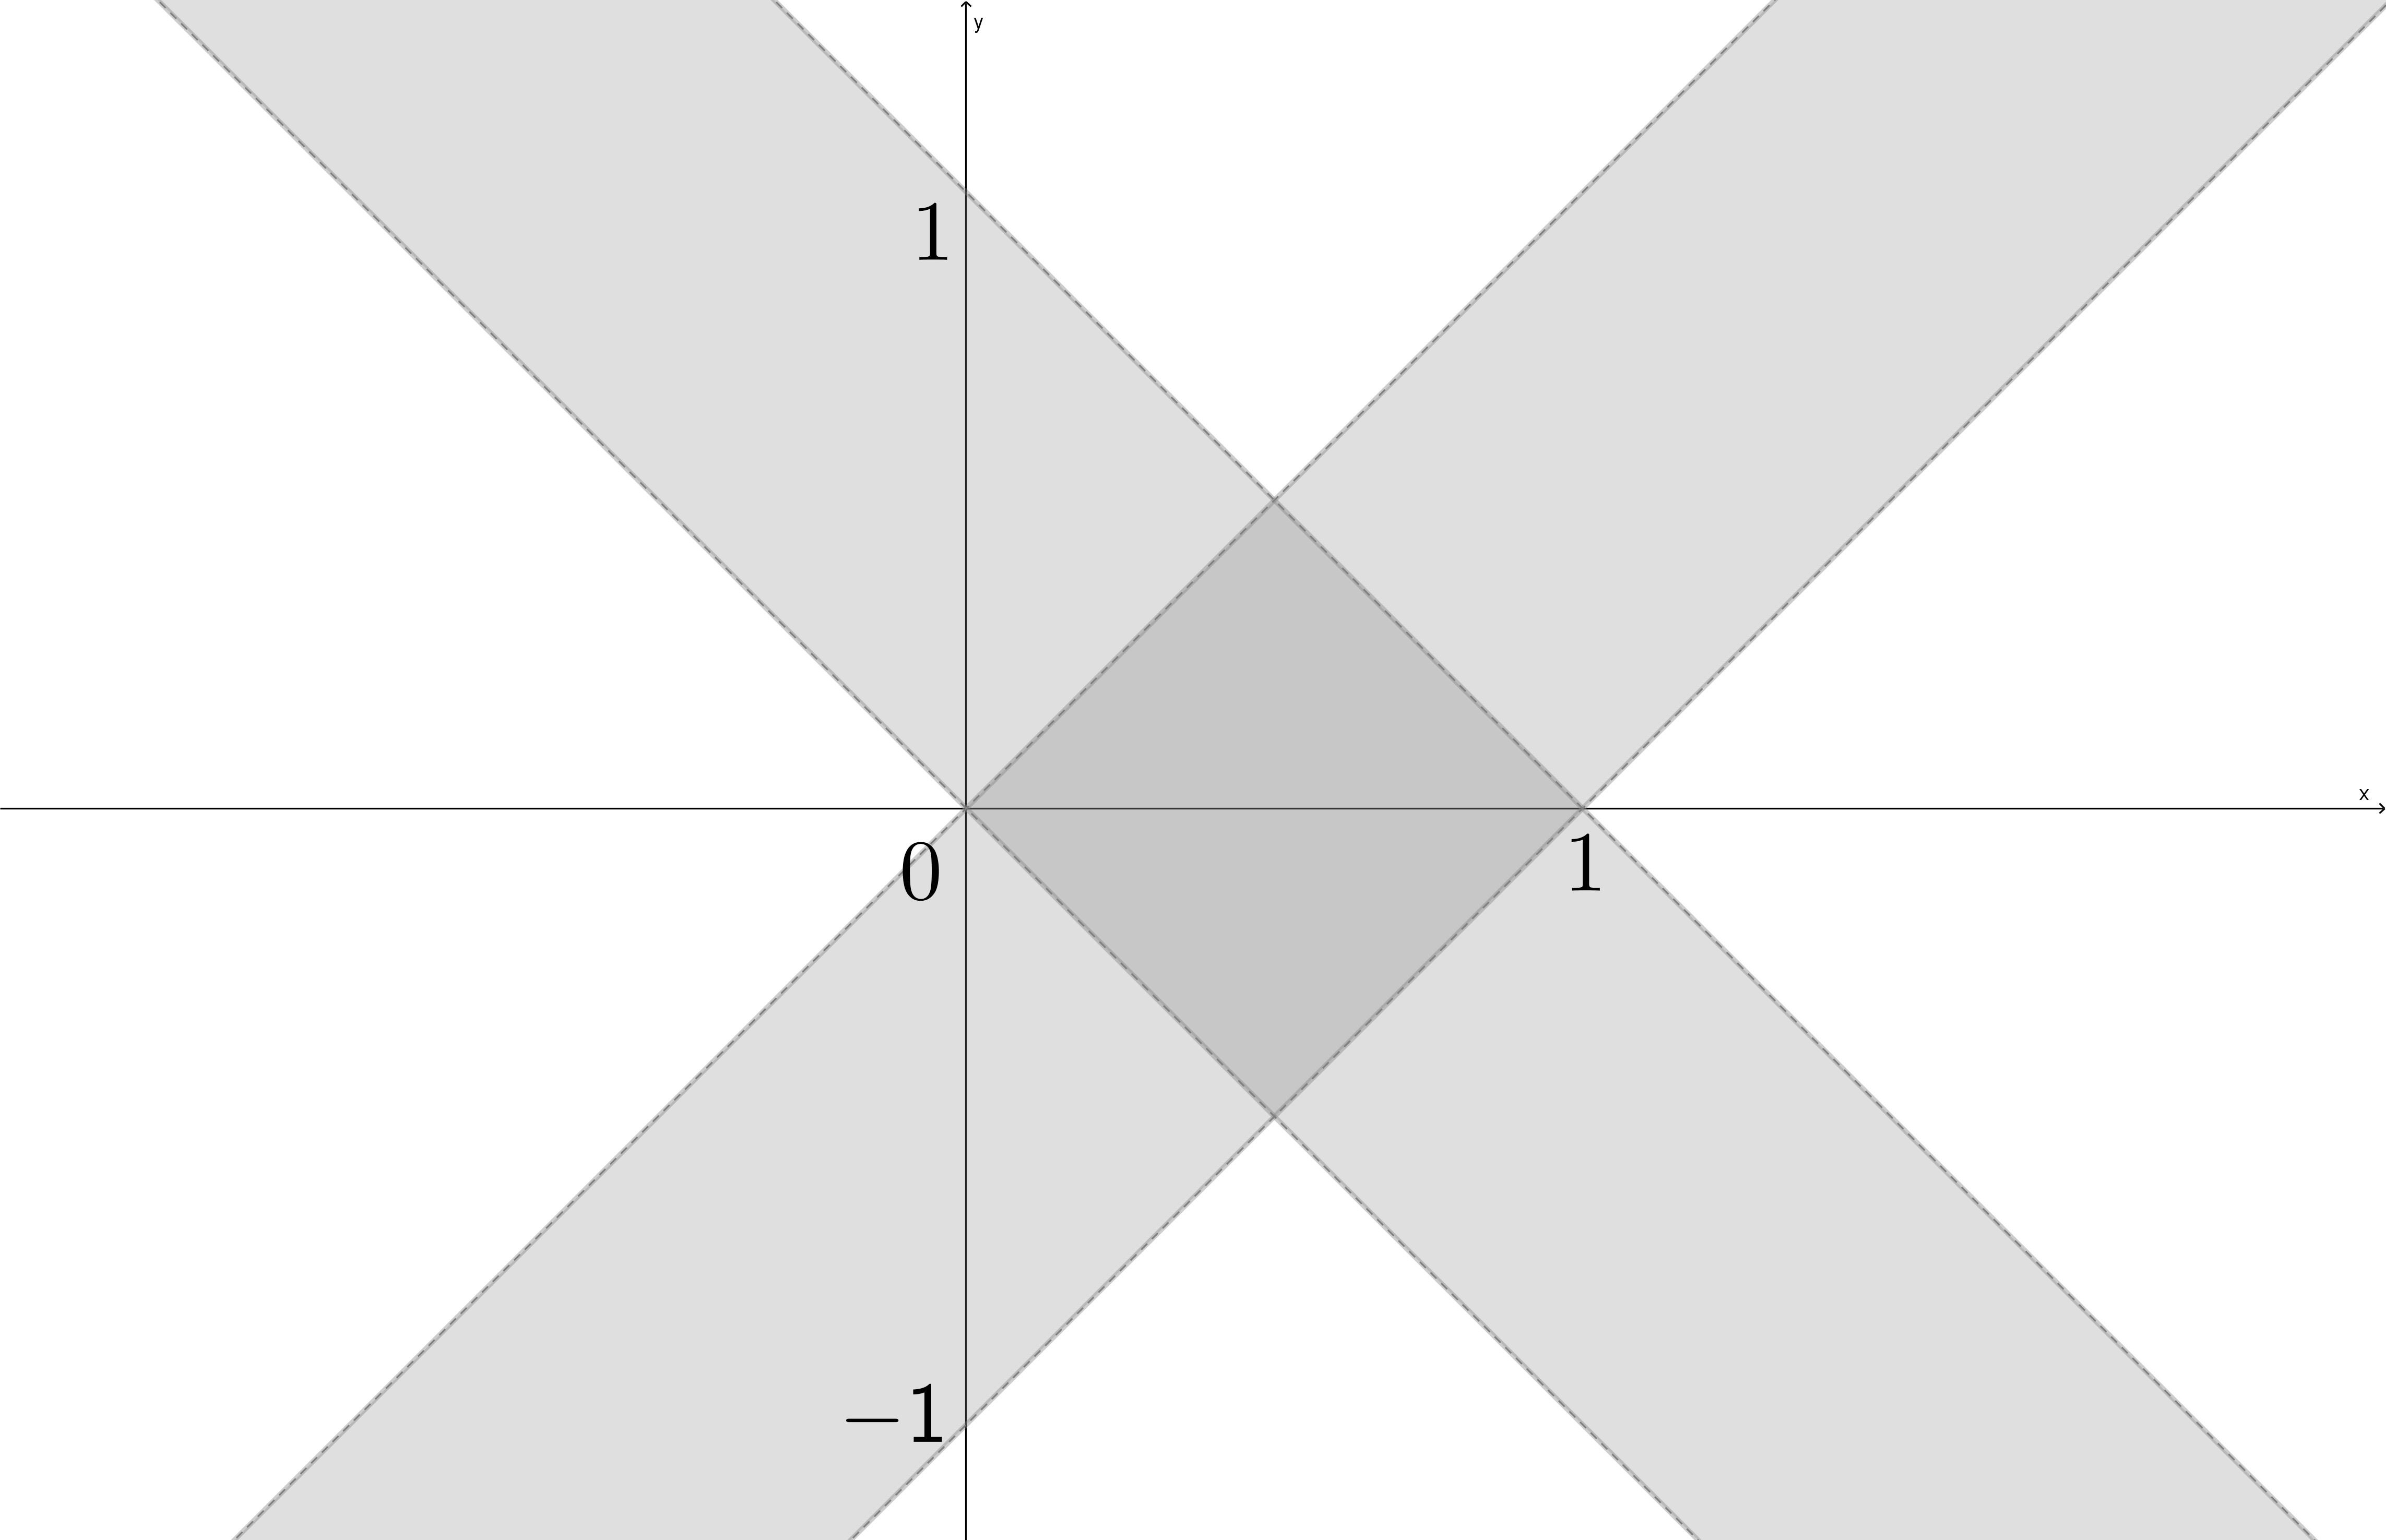
\includegraphics[width=70mm,bb  = 0 0 300 200]{31.png}
	\end{center}
 	\caption{積分領域$D$}
\end{minipage}
\begin{minipage}{0.5\hsize}
	\begin{center}
		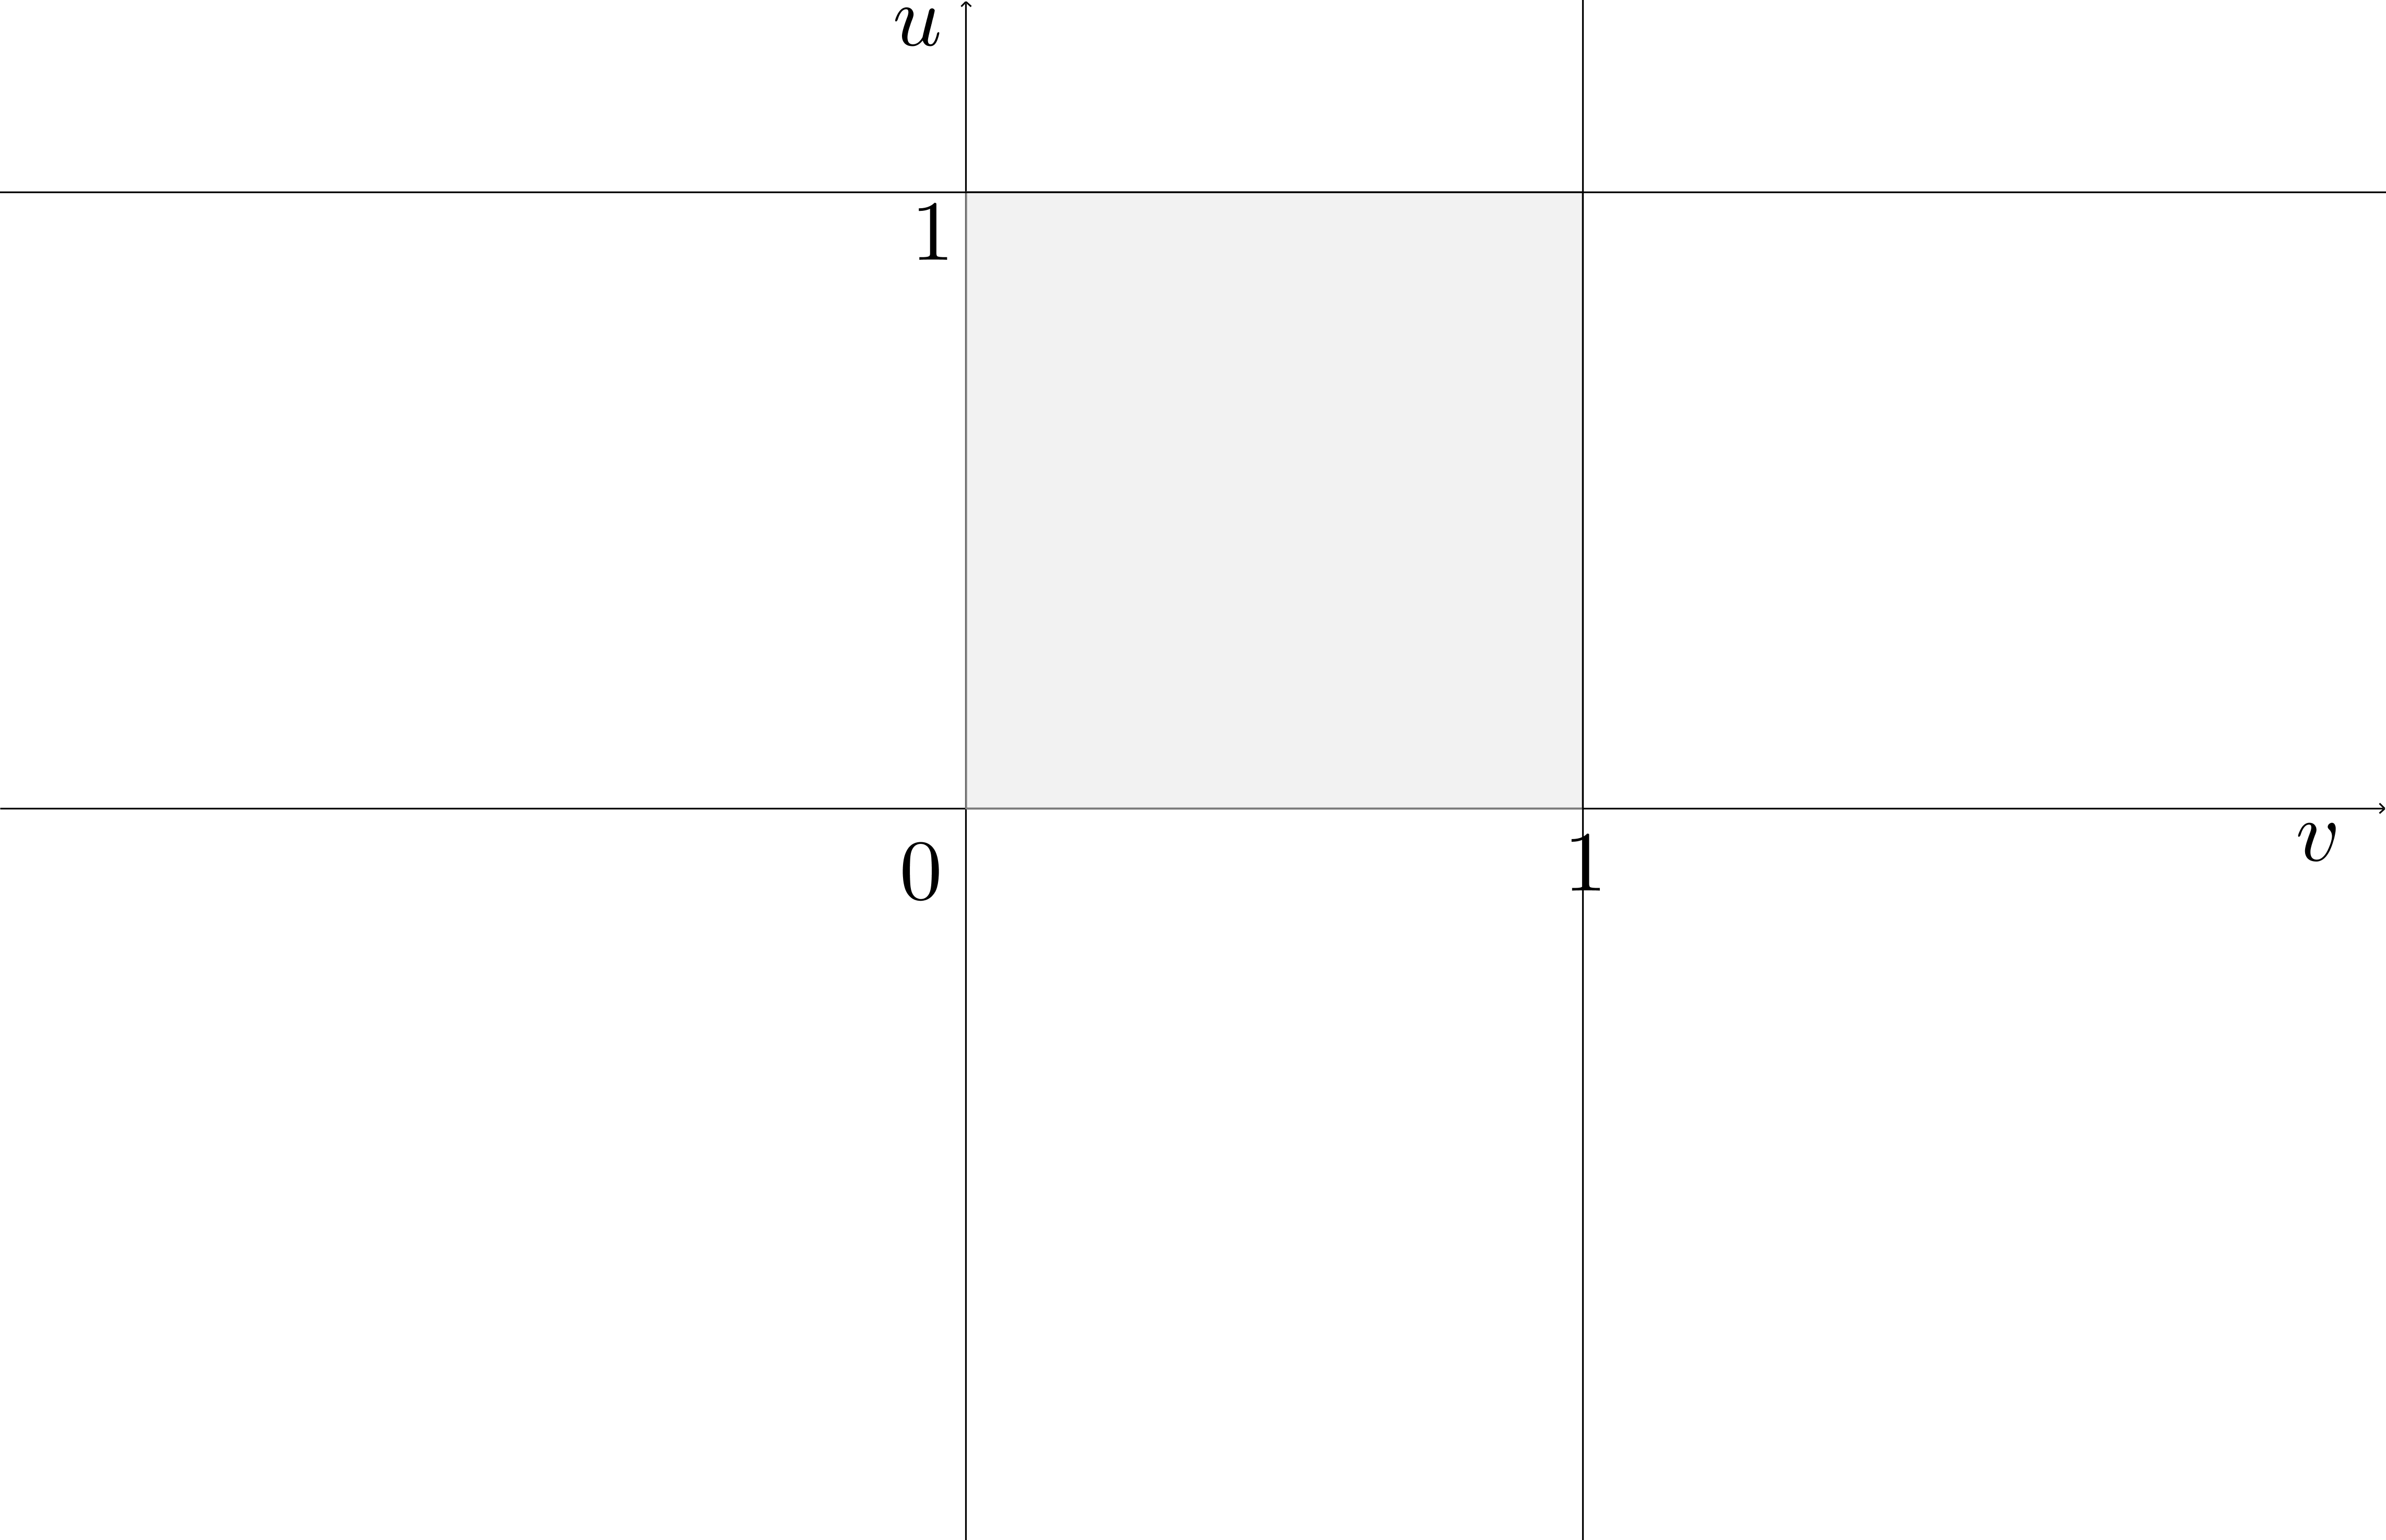
\includegraphics[width=70mm,bb  = 0 0 300 200]{32.png}
	\end{center}
	\caption{積分領域$E$}
\end{minipage}
\end{figure}

\item$ I = \iint_{D} (x-y)\log{(x+y+1)}dxdy $を求めよ

線形変換
\begin{fleqn}[30pt] \begin{gather*}
 	\left[ \begin{array}{r}
		u \\
		v \\
	\end{array}  \right]
	= \varphi(x,y)=
 	\left[ \begin{array}{r}
		x+y \\
		x-y \\
	\end{array}  \right]
	=
 	\left[ \begin{array}{cc}
		1 & 1 \\
		1 & -1 \\
	\end{array}  \right]
 	\left[ \begin{array}{r}
		x \\
		y \\
	\end{array}  \right]
\end{gather*} \end{fleqn}
は,
\begin{fleqn}[30pt] \begin{gather*}
	\rm{det}
 	\left[ \begin{array}{cc}
		1 & 1 \\
		1 & -1 \\
	\end{array}  \right]
	=1(-1)-1^2=^2 \ne 0
\end{gather*} \end{fleqn}
より線形同型であって,逆変換は
\begin{fleqn}[30pt] \begin{gather*}
	\det
 	\left[ \begin{array}{cc}
		1 & 1 \\
		1 & -1 \\
	\end{array}  \right]^{-1}
 	\left[ \begin{array}{r}
		u \\
		v \\
	\end{array}  \right]
	=\frac{1}{-2}
 	\left[ \begin{array}{cc}
		-1 & -1 \\
		-1 & 1 \\
	\end{array}  \right]
 	\left[ \begin{array}{r}
		u \\
		v \\
	\end{array}  \right]
	=\frac{1}{2}
 	\left[ \begin{array}{cc}
		1 & 1 \\
		1 & -1 \\
	\end{array}  \right]
 	\left[ \begin{array}{r}
		u \\
		v \\
	\end{array}  \right]
\end{gather*} \end{fleqn}
である.よって,そのJacobi行列式の絶対値は
\begin{fleqn}[30pt] \begin{gather*}
	|\det (\varphi^{-1})'(u,v)|=\left| \left(\frac{1}{2}\right)^2 \rm{det}
 	\left[ \begin{array}{cc}
		1 & 1 \\
		1 & -1 \\
	\end{array}  \right]
	\right| = \frac{1}{2}
\end{gather*} \end{fleqn}
であり,
\begin{fleqn}[30pt] \begin{gather*}
	(x,y) \in D \iff (u,v) \in E = \{ (u,v) \in \mathbb{R}^2 | 0 \leq u \leq 1, 0 \leq v \leq 1 \}
\end{gather*} \end{fleqn}
だから,
\begin{fleqn}[30pt] \begin{gather*}
	\iint_{D} (x-y)\log{(x+y+1)}dxdy\\
	= \iint_{E} v\log(u+1) \frac{1}{2}dudv\\
	= \frac{1}{2} \int^1_0 v \, dv \, \int^1_0\log(u+1)du\\
	= \frac{1}{2} \left[ \frac{1}{2} v^2 \right]^1_0 \left( \left[ u\log(u+1)\right]^1_0 - \int^1_0 \frac{1}{u+1} du \right) \\
	= \frac{1}{2} \frac{1}{2} \left( \log{2} - \left[ u - \log{u+1} \right]^1_0 \right) \\
	= \frac{1}{4} \left( \log{2} - (1-\log{2})\right)\\
	= \frac{1}{4} \left(2\log{2} - 1 \right)
\end{gather*} \end{fleqn}
\end{enumerate}

\newpage
%4
\section{次の各問いに答えよ.}
\begin{enumerate}
\item $ D=\{(x,y) \in \mathbb{R}^2 | x^2+y^2 \leq x\}$を図示せよ。なお(2)で変数変換を用いる場合は新たな積分領域も描け。
\begin{figure}[h]\begin{minipage}{0.5\hsize}
	\begin{center}
		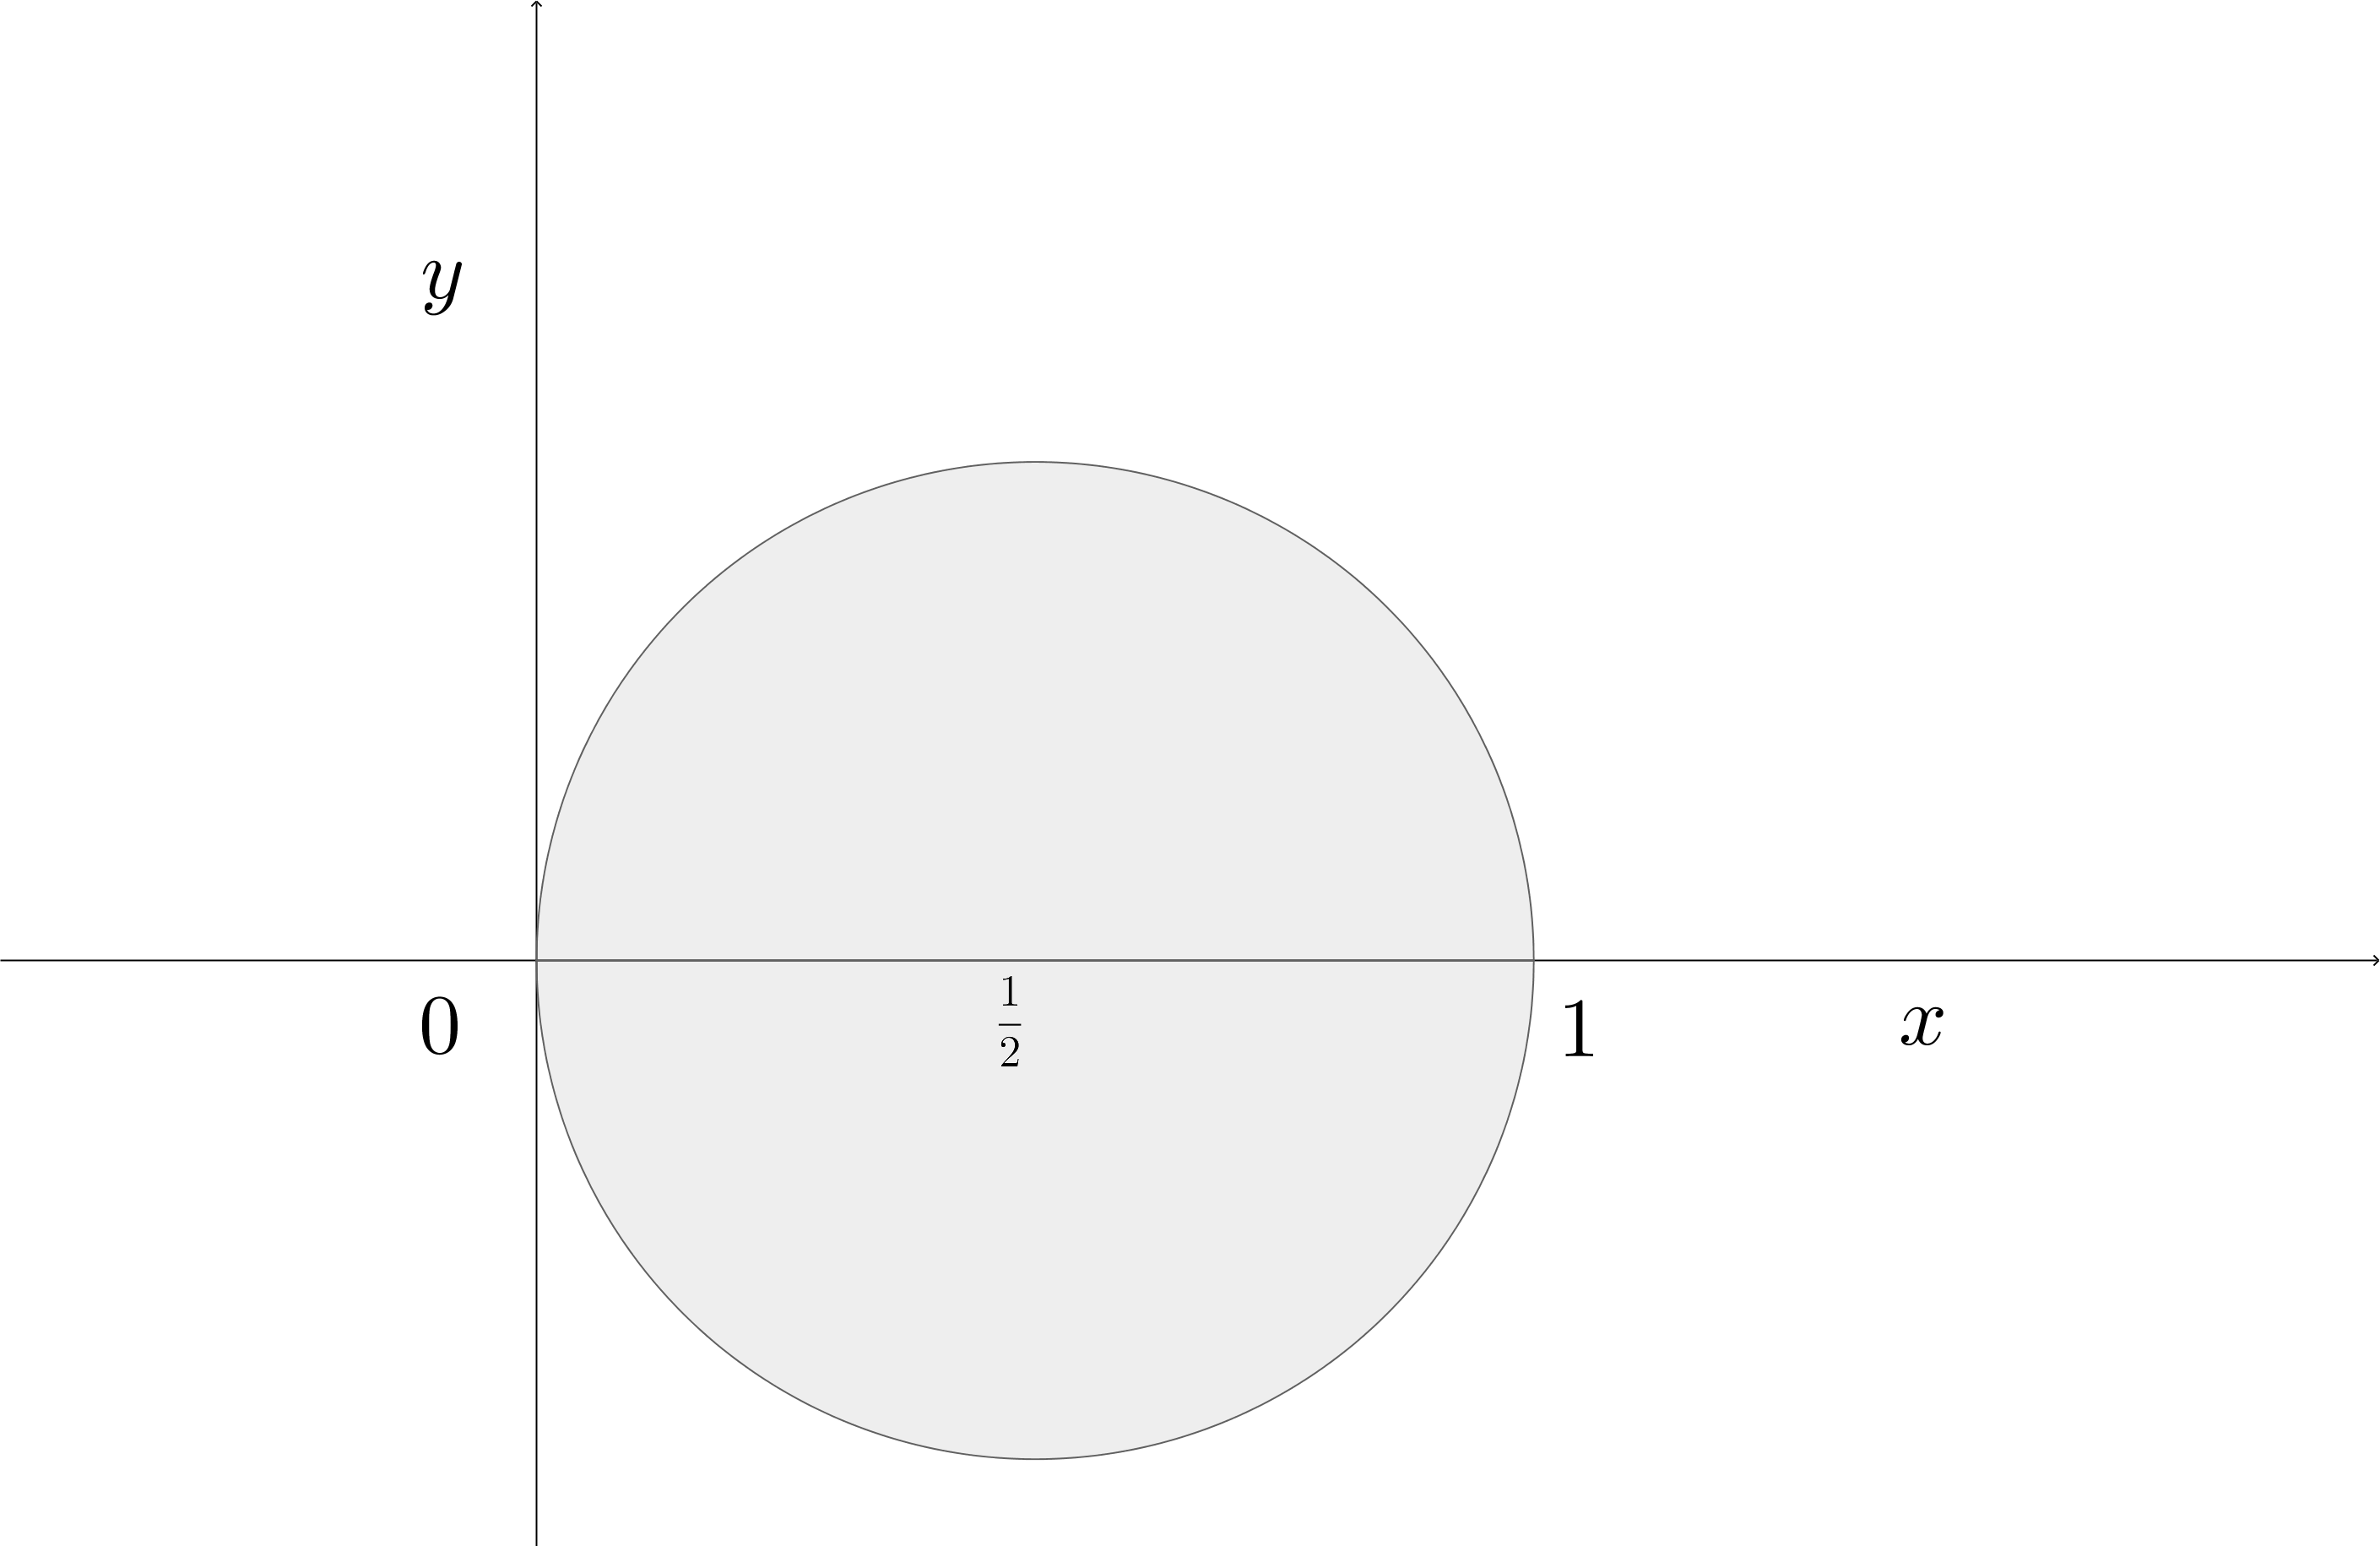
\includegraphics[width=70mm,bb  = 0 0 300 200]{41.png}
	\end{center}
 	\caption{積分領域$D$}
\end{minipage}
\begin{minipage}{0.5\hsize}
	\begin{center}
		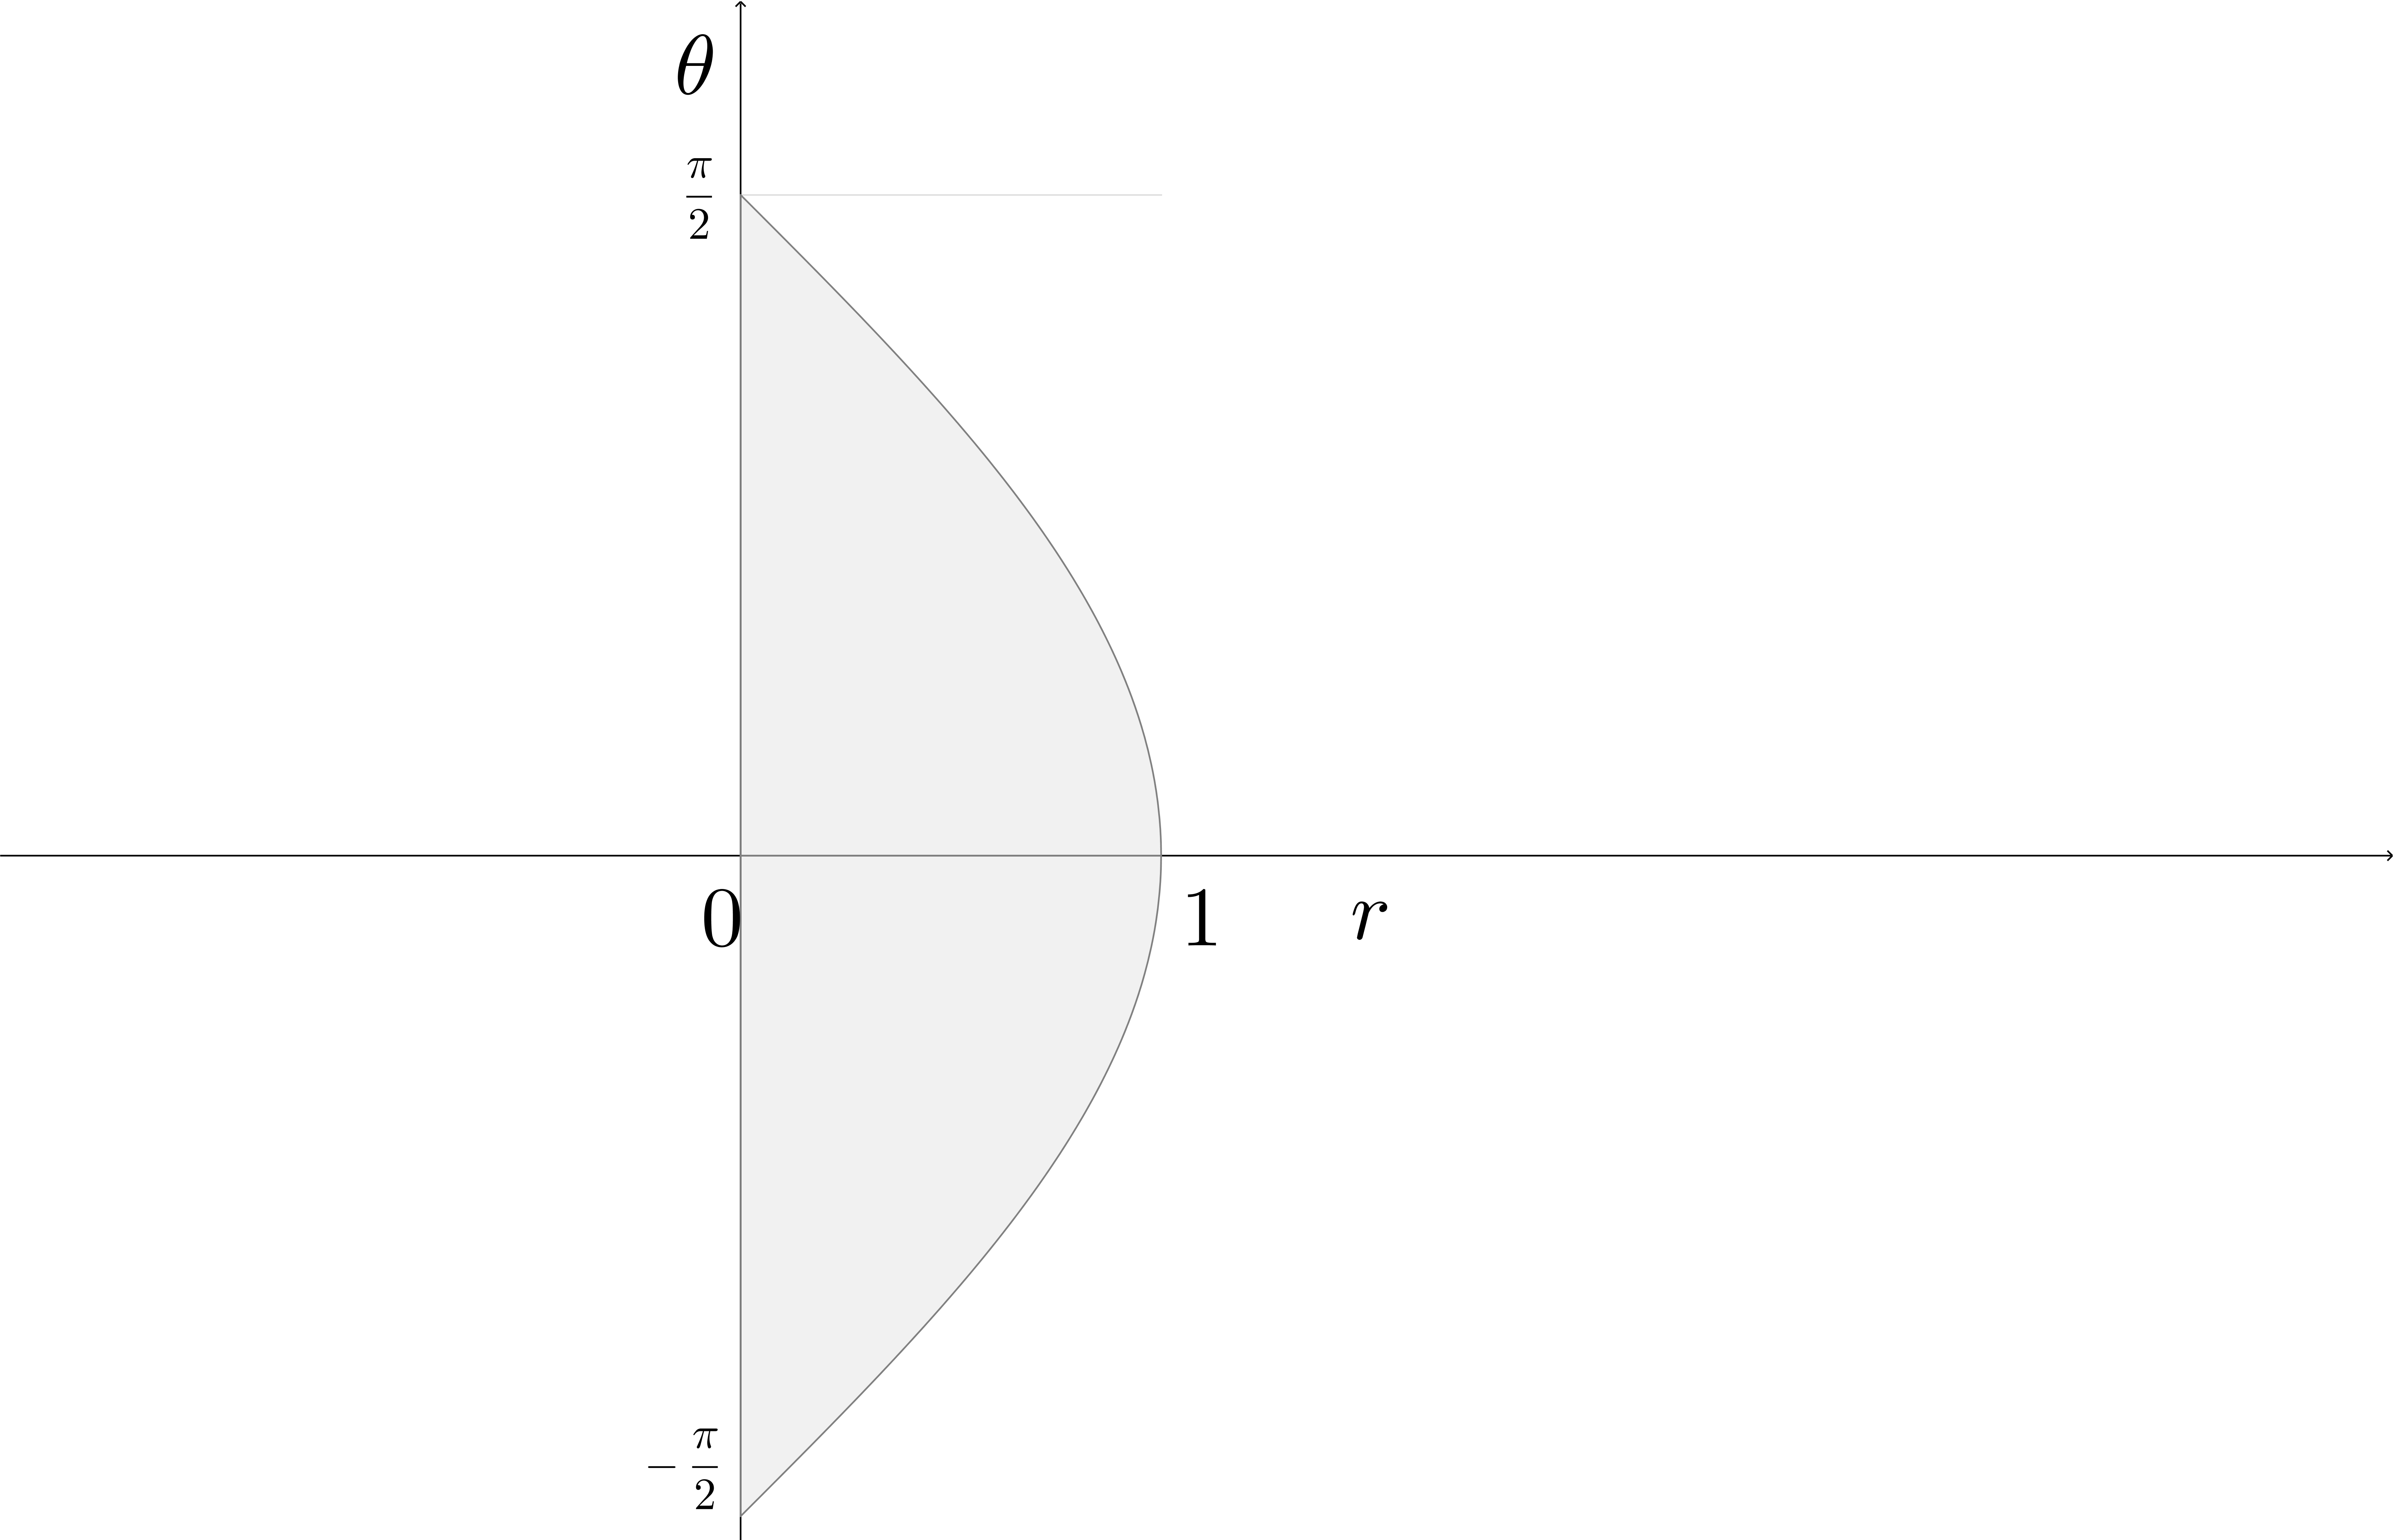
\includegraphics[width=70mm,bb  = 0 0 300 200]{42.png}
	\end{center}
	\caption{積分領域$E$}
\end{minipage}
\end{figure}
\item$ I=\iint_{D} \sqrt{1-x^2-y^2}dxdy$を求めよ

極座標変換
\begin{fleqn}[30pt] \begin{gather*}
 	\left[ \begin{array}{r}
		x \\
		y \\
	\end{array}  \right]
	= r
 	\left[ \begin{array}{r}
		\cos{\theta} \\
		\sin{\theta} \\
	\end{array}  \right]
	,\quad r \geq 0 , \quad -\frac{\pi}{2} \leq \theta \leq \frac{\pi}{2}
\end{gather*} \end{fleqn}
によって$r\theta$平面の領域$E$が$xy$平面上の領域$D$に1対1にうつります.
\begin{fleqn}[30pt] \begin{gather*}
	\iint_{D} \sqrt{1-x^2-y^2}dxdy \\
	=\int^{\frac{\pi}{2}}_{-\frac{\pi}{2}} \int^{\cos{\theta}}_0 \sqrt{1-r^2\cos{\theta}-r^2\sin{\theta}} r dr d\theta\\
	=\int^{\frac{\pi}{2}}_{-\frac{\pi}{2}} \int^{\cos{\theta}}_0 r\sqrt{1-r^2} drd\theta
\end{gather*} \end{fleqn}
ここで,
\begin{fleqn}[60pt] \begin{gather*}
	t=\sqrt{1-r^2} \qquad
	dt=-\cfrac{r}{2t}dr \qquad
	\begin{array}{c|r}
		r & 0 \to \cos{\theta} \\ \hline
		t & 1 \to \sin{\theta}
	\end{array}
\end{gather*} \end{fleqn}
\begin{fleqn}[30pt] \begin{gather*}
	=\int^{\frac{\pi}{2}}_{-\frac{\pi}{2}} \int^{\sin{\theta}}_1 r \cdot t \frac{-2t}{r} dt d\theta\\
	=-2 \int^{\frac{\pi}{2}}_{-\frac{\pi}{2}} \left[ \frac{1}{3}t^3 \right]^{\sin{\theta}}_1 d\theta \\
	=-\frac{2}{3} \int^{\frac{\pi}{2}}_{-\frac{\pi}{2}} ( \sin^3{\theta} - 1 ) d\theta \\
	= -\frac{2}{3} 2\int^{\frac{\pi}{2}}_{0}  ( \sin^3{\theta} - 1 ) d\theta \\
	=-\frac{2}{3} \left( \frac{2}{3} - \frac{\pi}{2} \right) \\
	= \frac{\pi}{3}- \frac{4}{9}
\end{gather*} \end{fleqn}
\end{enumerate}

\end{document}
